%!TEX root = ../../thesis.tex
%!TEX enableSynctex = true
%*******************************************************************************
%****************************** Third Chapter **********************************
%*******************************************************************************
% **************************** Define Graphics Path **************************
\ifpdf
    \graphicspath{{Chapters/flopt/Figs/Raster/}{Chapters/flopt/Figs/PDF/}{Chapters/flopt/Figs/}}
\else
    \graphicspath{{Chapters/flopt/Figs/Vector/}{Chapters/flopt/Figs/}}
\fi

\chapter{Frame Localisation Optical Projection Tomography}

Orthogonal imaging schema can be replaced with pass through imaging provide samples are sufficiently transparent.
Instead of scanning these samples lateral one can rotate their sample and reconstruct a full three dimensional image.
This chapter addresses a key downside in traditional approaches to performing full three dimensional reconstructions tomographically.
As tomographic technology has been shrunk to the millimeter scale, errors induced by hardware become apparent.
An algorithm will be presented that relies exclusively on multiple (5>) tracked fiducially beads and reconstructs without relying on any conic fitting on said beads.
The algorithm presented will use an extension projective mathematics discussed in Chapter %TODO insert chapter.


\section{Tomography (Pedro)}
Three-dimensional imaging of anatomy in thick biological samples provides valuable data for developmental biology studies.
Tomographic techniques that generate 3D reconstructions from 2D images such as computed tomography (CT) and magnetic resonance imaging (MRI) are essential in medical applications to visualize morphology in large tissues and organs.
CT and especially micro-CT can achieve micron-scale resolution using certain contrast agents, however the high doses of radiation used make this unsuitable for repeated experiments on a biological sample.
Micro-MRI can also achieve resolution in the micron scale, however the cost and size of MRI instruments can be prohibitive for many applications[21].
Furthermore, neither of these techniques can exploit the plethora of information that can be extracted through fluorescence microscopy.

Optical Projection Tomography was first proposed by Sharpe in 2002 [30]; it uses visible light to image and create volumetric data of transparent (naturally or artificially) mesoscopic objects (1 - 10 mm) at micron-level resolution.
OPT is based on well-documented computerized tomography techniques [17] in which a set of images (we will refer to these as projections) of an object are acquired with a camera at discrete steps over a full rotation.
A cross-sectional stack of slices from the original object is reconstructed using a back-projection algorithm from the projection images.
OPT is non-invasive (although it may require fixed samples), and it can image in two different modalities: emission OPT (eOPT) and transmission OPT (tOPT).
In eOPT, a fluorescent sample is excited using a wide-field illumination source.
The photons emitted by a fluorophore of interest are collected by a detector with an appropriate filter to reject the incident illumination.
In tOPT, a broadband source with a diffuser and a collimator lens located on the optical axis (as shown in figure 1) directs quasi-collimated, uniform illumination onto the sample.
The intensity collected at the camera is a function the amount of light absorbed by the sample.
In other words, the image recorded by the detector is a projection of the attenuated radiation that traverses the sample.
These two modalities can work together to display fluorescent signals in the context of the whole organism anatomy.
OPT attempts to address the scale gap between the tomographic techniques described above (samples larger than 10 mm), and light microscopy techniques (samples smaller than 1 mm) to image biological samples in the 1-10 mm regime.

\begin{figure}
  \centering
  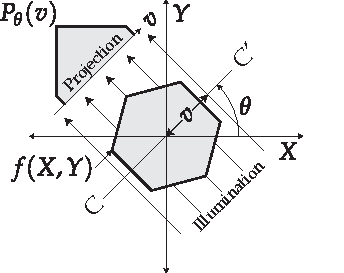
\includegraphics{Chapters/flopt/Figs/PDF/OPT_digram}
  \caption{Principle of OPT, a respective rotation between the sample and the detector illumination pair is iterated, the volumetric image is later reconstructed.}
\end{figure}

\subsection{Reconstruction}

Photons from an illumination source impinge on the sample and are attenuated as they traverse the volume of the sample towards a detector.
The detector collects a series of intensity profiles $I = I_{I}e^{-k}$ at discrete angular steps $n$ through a full rotation of the sample, where $I_{\theta}$ is the unattenuated radiation intensity from the source to the detector.
$k$ is the attenuation from all the voxels along the trajectory of a single ray, and $I$ is the measured intensity (shown in figure 3).
As mentioned in section 1, the rays from the sample to the detector approximate straight lines when their angular extent is small, so we can approximate the rays reaching the detector with line integrals.
The resulting intensity profile at the detector for a particular rotation angle is a projection, and the integral transform that results in $f(I_i,\theta_n)$ is the Radon transform.
This is defined mathematically as:
\begin{align}
    f(I,\theta) = \int \int R(x,y)\delta (xcos(\theta)+y sin(\theta)-I)dx dy
\end{align}
where $f(I,\theta)$ is the Radon transform, is the unit impulse, and $R(x,y)$  represents a 2D slice of the sample.
A parallel projection is then just the combination of line integrals $f(I)$ for a constant.% for a constant.
An inverse Radon transform is used to recover the original object from the projection data; filtered back-projection (FBP) is a standard and popular method to achieve this inversion [17].
The key behind FBP is to use the Fourier transform of each projection measurement to reorder the information from the sample onto its original place in the Fourier domain, and then take the inverse transform to recover the shape of the sample.
This is derived from the Fourier Slice Theorem [17], which states that the one-dimensional Fourier transform of a parallel projection is equivalent to a slice of the two-dimensional Fourier transform of the original object.
A filtering step is applied during back-projection to avoid spatial frequency oversampling during the object’s rotation (this
is shown in figure 5).
A high pass filter such as a ramp filter is commonly used to counter the blurring caused by this oversampling.
FBP be thought of as smearing the projection data across the image plane, and is expressed in equation form as:
\begin{align}
R_{fpb}(x,y) = \int_{0}^{\pi} f'(x\cos(\theta)+y\sin(\theta),\theta)dxdy
\intertext{where $f'$ is the filtered projection data, and $R_{fbp}$ is the back-projected image.}
\end{align}

\subsubsection{Aim}


\section{Stereoscopic Imaging}

\subsection{Projective geometry}

Camera imaging is governed by projective geometry
Parallel lines project onto a camera will have a vanishing points

\subsection{Camera projections}

\subsection{Multiple view scenes}
Have two views allows us to triangulate from features or fudicials in one camera to another.
Triangulation requires features in both images to be the same, this is known as the correspondence problem

Suppose we know the relative positions of the cameras and their intrinsic parameters.
Given the CCD parameters, we can translate pixel coordinates (u, v) into image plane coordinates $(x, y)$:
\begin{align}
    u = u_0 + k_u x
    v = v_0 + k_v y
\end{align}

With the focal length, image plane coordinates can be translated into a ray in 3D.
The ray may be defined by the point $\textbf{p}$ in the camera-centred coordinates where it pierces the image plane:

\subsubsection{Epipolar geoemtry}
An important part of stereo is triangulating 2 rays from a pair of image correspondences.
The most important matching constraint which can is used is the epipolar constraint, and follows directly from the fact that the rays must intersect in 3D space.
Epipolar constraints facilitate the search for correspondences, they constrain the search to a line in each image.
To derive general epipolar constraints, consider the epipolar geometry of two cameras:

The baseline is the line joining the optical centres.
An epipole is the point of intersection of the baseline with the image plane.
There are two epipoles, one for each image.
An epipolar line is a line of intersection of the epipolar plane with an image plane.
It is the image in one camera of the ray from the other camera’s optical centre to the point $X$.
For different world points $X$, the epipolar plane rotates about the baseline.
All epipolar lines intersectat the epipole.

The epipolar line constrains the search for correspondence from a region to a line.
If a point feature $\textbf{x}$ is observed in one image, then its location $\textbf{x'}$ in the other image must lie on the epipolar line.
We can derive an expression for the epipolar line.
The two camera-centered coordinate systems are related by a rotation $R$ and translation $\textbf{T}$:

\begin{align}
    \mathbf{X'}_c &= R\mathbf{X'}_c + \mathbf{T} \nonumber \\
    \intertext{Taking the vector product with T, we obtain} \nonumber \\
    T \times \mathbf{X'}_c &= T \times R\mathbf{X'}_c + \mathbf{T} \times \mathbf{T} \nonumber \\
    T \times \mathbf{X'}_c &= T \times R\mathbf{X'}_c \label{Xprime = RTX}
\end{align}

\begin{figure}
  \centering
  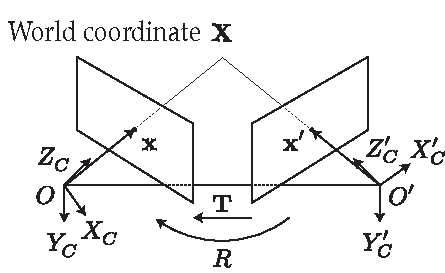
\includegraphics{Chapters/flopt/Figs/PDF/epi-polar-geom}
  \caption{Epi-polar geometry described for two adjacent views (or cameras of a scene).}
\end{figure}

\subsubsection{Essential Matrix}

Taking the scalar product with $\mathbf{X'_c}$, we obtain:
\begin{align}
    \mathbf{X'}_c \cdot (\mathbf{T} \times \mathbf{X'}_c) &= \mathbf{X'}_c\cdot (\mathbf{T} \times R\mathbf{X'}_c)\nonumber \\
    \mathbf{X'}_c \cdot (\mathbf{T} \times R\mathbf{X'}_c) &= 0 \nonumber
\end{align}
A vector product can be expressed as a matrix multiplication:
\begin{align}
T \times \mathbf{X}_c &= T_\times \mathbf{X}_c \\
\intertext{where}
T_\times &=\begin{bmatrix}
0    & -T_z  & T_y\\
T_z  & 0     & -T_x\\
-T_y  & T_x   & 0
\end{bmatrix}
\end{align}
So equation \eqref{eq:Xprime = RTX} can be rewritten as:

\begin{align}
\mathbf{X'}_c \cdot (T_\times R\mathbf{X}_c) = 0 \nonumber\\
\mathbf{X'}_c T E \mathbf{X}_c = 0  \nonumber\\
\intertext{where}  \nonumber\\
E = T_\times R \nonumber
\end{align}

E is a $3 \ times 3$ matrix known as the \emph{essential matrix}.
The constraint also holds for rays $\mathbf{p}$, which are parallel to the camera-centered position vectors $\mathbf{X}_c$:

\begin{align}
\mathbf{p}'^T E \mathbf{p} = 0 \label{eq:pEp}
\end{align}
This is the epipolar constraint.
If we observe a point $\mathbf{p}$ in one image, then its position $\mathbf{p'}$ in the other image must lie on the line defined by \eqref{eq:pEp}.
The essential matrix can convert from pixels to rays $\mathbf{p}$ assuming a calibrated camera.
And pixel coordinates can be converted to image plane coordinates using:
\begin{align}
\begin{bmatrix}
u\\
v\\
1
\end{bmatrix}
&=
\begin{bmatrix}
k_u & 0 & u_0 \\
0 & k_v & v_0 \\
0 & 0 & 1
\end{bmatrix}
\begin{bmatrix}
x\\
y\\
1
\end{bmatrix}
\intertext{We can modify this to derive a relationship between pixel coordinates and rays:}
\begin{bmatrix}
u\\
v\\
1
\end{bmatrix}
&=
\begin{bmatrix}
\frac{k_u}{f} & 0 & \frac{u_0}{f} \\
0 & \frac{k_v}{f} & \frac{v_0}{f} \\
0 & 0 & \frac{1}{f}
\end{bmatrix}
\begin{bmatrix}
x\\
y\\
f
\end{bmatrix}
\intertext{If we define the matrix $K$ as follows:}
K &= \begin{bmatrix}
f k_u & 0 & u_0 \\
0 & f k_v & v_0 \\
0 & 0 & 1
\end{bmatrix}
\intertext{then we can write}
\mathbf{\widetilde{w}} &= K\mathbf{p}
\end{align}

\subsubsection{Fundamental Matrix}

\begin{align}
    \intertext{The epipolar constraint becomes}\\
    \mathbf{p'}^T E \mathbf{p} &= 0 \\
    \mathbf{\widetilde{w'}}^T K^{-T} E K^{-1} \mathbf{\widetilde{w}} &= 0 \\
    \mathbf{\widetilde{w'}}^T F \mathbf{\widetilde{w}} &= 0
\end{align}

F is the $3\times3$ \emph{fundamental matrix}.

%\subsubsection{Two views}
%\paragraph{Mapping from one camera to another}
%\subsubsection{Three and more views}

With intrinsically calibrated cameras, structured can be recovered by triangulation.
Firstly obtain the two projection matrices are obtained via a singular value decomposition of the essential matrix.
The SVD of the essential matrix is given by:

\begin{align}
    \hat{T}_{\times} = U \begin{bmatrix}
    0 & 1 & 0 \\
    -1 & 0 & 0 \\
    0 & 0 & 0
    \end{bmatrix} U^T
    &\text{ and }
    R = U \begin{bmatrix}
    0 & -1 & 0 \\
    1 & 0 & 0 \\
    0 & 0 & 1
    \end{bmatrix} V^T
    \intertext{Then, aligning the left camera and world coordinate
    systems:}
    P = K [I | \mathbf{0}]
    &\text{ and }
    P' = ' [R | \mathbf{T}]
\end{align}

Given the two projection matrices, we can recover structure (only up to scale, since $|\mathbf{T}|$ is unknown) using least squares.
Ambiguities in $\mathbf{T}$ and R are resolved by ensuring that visible points lie in front of the two cameras.
As with the essential matrix, the fundamental matrix can be factorised into a skew-symmetric matrix corresponding
to translation and a 3 × 3 non-singular matrix corresponding to rotation.

\section{The new algorithm}

The rotation may also not be orthogonal to the plane of detection.
An observer will notice the trajectory of a fiducial following a conic section, usually an ellipse.
During an OPT reconstruction there will be a fitting step to recover ellipse and to correct for it before applying a radon transform.
This type of reconstruction not only ignores any mechanical jitter of the sample but also the possibility of a systematic drift.

We have seen however that using two adjacent images of a scene, points may be triangulated within the scene given the rotational and translational matrices of the respect camera views.
The inverse is also possible given a sufficient amount of reliable fiducial points in a scene.
The recovery over a more exact description of the motion of the scene can eliminate any need for a fitting, recover and correct for drift as well as eliminate any mechanical jitter.
Errors may then be introduced from fiducially mechanically slipping and localisation errors.

Using the factorisation of the Fundamental, Essential or Homography matrix each adjacent view of a rotating scene can have it's translation and rotational matrices recovered.
Here we will discuss a reconstruction using $F$ but the same principle applies for $E$ and $H$.

\begin{figure}
  \centering
  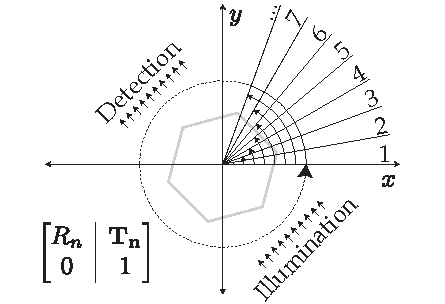
\includegraphics{Chapters/flopt/Figs/PDF/flOPT_principle}
  \caption{Each iteration during an OPT acquisition will have an associate $R$ and $\mathbf{T}$, these matrices can be recovered from comparing the current iteration to the previously iteration.}
\end{figure}

There are two ways of reconstructing using matrix as described above.
The first method involves computing F for two neighbouring images with 5 or more fiducials to remove ambiguity.
Once F is calculated F is decomposed into $R_n$ and $T_n$ between each view $n$ and $n+1$.
The image at view $n+1$ is then back projected to create a volume, the size is chosen to be suitably large (so that important data is not lost).
Then all the prior rotation and translation matrices are series multiplied until until $R_n$ and $T_n$, this final matrix is inverted and applied to the back projected volume.
This process is repeated for every angle and the back projected volume from each step is summed with every other step.
Finally the remaining volume is filtered using a Ram-Lak filter \footnote{Linear ramp filter in Fourier space: $|v|$},
By producing a series of of transformation matrices errors compound and the reconstruction of volumes degrades with more projections, see Figure \ref{fig:irandons}.

The second method is more robust.
Instead of calculating F between neighbouring images F is calculated between the current projection and the very first projection.
F is then decomposed and the transformation matrix is inverted and applied to the back projected volume.
The reoriented back projected volumes and summed as before and filtered.

\begin{figure}
  \centering
  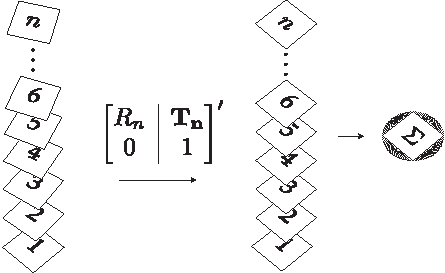
\includegraphics{Chapters/flopt/Figs/PDF/flopt_algorithm}
  \caption{Two dimensional representation of the reconstruction algorithm.
  The rotational and translation matrices are recovered and inversely applied to back projected images.
  The now realigned back projection are summated to produce an unfiltered back projection.}
\end{figure}

The second approach may be robust to compound errors but an additional programatic step is needed is know which beads in the first image correspond to beads in the current image.
This can be is achieved using standard tracking and momentum particle tracking algorithms [cite].
In both cases a decomposed F will produce 4 possible transformation pairs %(R,T; R,-T; -R,T; -R,-T) %TODO look this up.
are produced.
Once the first two views' transformation matrix is calculated the follows matrices can be chosen by likelihood or even subtracting \([Rn|Tn]\) from \(Rn-1|Tn-1\) and minimising.
The first two views are more difficult to choose the correct decomposition for but it is possible if a suitable ideal matrix is given as a comparison.

\subsection{Results}

To verify the proposed algorithm works, it was applied to simulated data.
The image of Lena
\footnote{The image of Lena is used as a reference to a very early full colour digital scanner.
The researchers in question realised that their presentation of the scanner's capabilities at a conference lacked a test image.
The nearest image to hand was a Playboy magazine with Lena Söderberg as the centrefold.}
is used here as a test image to verify the validity of each reconstruction.
Superimposed on Lena are fiducial beads to track the rotation of the image, see Figure \ref{fig:raw_input}.
The reference image was then rotated through 128 angles over $2\pi$ radians of rotation and projected along the $y$ axis to create a single line projection.
This is repeated for each angle with each line projection stacked to create a sinugram, see Figure \ref{fig:sinugram_stretch}.


\begin{figure}
  \centering
  \hfill
  \begin{subfigure}[t]{0.3\textwidth}
    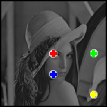
\includegraphics[width=\textwidth]{Chapters/flopt/Figs/PDF/results/no_helix/rawinput_colour}
    \caption{Raw input for OPT simulations, Lena.}
    \label{fig:raw_input}
  \end{subfigure}\hfill
  \begin{subfigure}[t]{0.3\textwidth}
    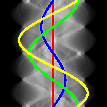
\includegraphics[width=\textwidth]{Chapters/flopt/Figs/PDF/results/no_helix/sinugram_stretch}
    \caption{Image of Lena (Figure \ref{fig:raw_input}) after rotation and projection in 2D, giving the sinugram.}
    \label{fig:sinugram}
  \end{subfigure}
  \hfill
  \label{fig:rawinputs}
  \caption{Reference images for OPT reconstruction.}
\end{figure}

In the standard algorithmic approach for OPT, the sinugram produced then undergoes the Radon transform, see Figure \ref{fig:iradon_nofilter} and then a post filtering, see Figure \ref{fig:iradon_nofilter}.
Instead of the the radon transform the proposed algorithm is used.
In Figure \ref{fig:flopt_comparison_line_profile} the two techniques are compared for ideal conditions of smooth, predictable rotation.
The proposed algorithm produces by eye (see Figure \ref{fig:flopt_filter}) a faithful reconstruction on the original image.
Both techniques however lose some of the original contrast of the image due to under-sampling of rotations.
However, the proposed algorithm fairs worse in terms of contrast compared to a Radon transform.

The case of a sample drifting systematically along the $x$ axis is now considered, this produces a helical path of a single fiducial within the sample.

In Figure \ref{} the Radon transform fails to reconstruct with a slight helically.
However, the proposed algorithm produces a similar result to that of a sample rotating without any systematic drift.


\begin{figure}
  \centering
  \hfill
  \begin{subfigure}[t]{0.3\textwidth}
    
\includegraphics[width=\textwidth]{Chapters/flopt/Figs/PDF/results/no_helix/iradon_nofilter}
    \caption{Unfiltered output of the radon transform}
    \label{fig:iradon_nofilter}
  \end{subfigure}\hfill
  \begin{subfigure}[t]{0.3\textwidth}
    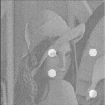
\includegraphics[width=\textwidth]{Chapters/flopt/Figs/PDF/results/no_helix/iradon_filter}
    \caption{Ram-lak (Fourier ramp) filter applied to Figure \ref{fig:iradon_nofilter}.}
    \label{fig:iradon_filter}
  \end{subfigure}
    \hfill
    \label{fig:irandons}
  \caption{The result of an Tomographic reconstruction requires Fourier filtering to normalise spatial contrast}
\end{figure}

\begin{figure}
  \centering
  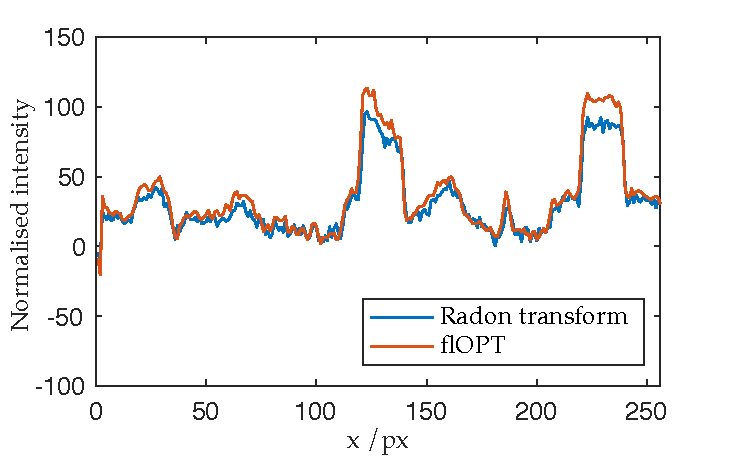
\includegraphics{Chapters/flopt/Figs/PDF/results/comparison_line_profile}
  \caption{Line profile comparison of the reconstruction of a reference image artificially rotated and projected using the standard radon transform and the new proposed algorithm.}
  \label{fig:flopt_comparison_line_profile}
\end{figure}

\begin{figure}
  \centering
  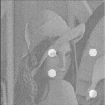
\includegraphics[width=0.3\textwidth]{Chapters/flopt/Figs/PDF/results/no_helix/flopt_filter}
\caption{Reconstruction of a reference image using the new proposed algorithm}
\label{fig:flopt_filter}
\end{figure}

The reconstruction algorithm was then applied to simulated OPT data with which a systematic drift was added.
The resulting path of a single bead then resembles a helix, and importantly, with a different start and finishing positions.
As shown in Figure (%todo insert figure)
) the radon transform approach falls down whilst the proposed algorithm performs as well as it did prior.
The path that any single bead draws out also could not be satisfactorily mapped to a conical section to characterise the motion observed.


\begin{figure}
  \centering
  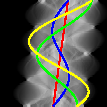
\includegraphics[width=0.3\textwidth]{Chapters/flopt/Figs/PDF/results/helix/sinugram_stretch}
\caption{Sinugram of a sample whose axis of rotation has a systematic drift}
\label{fig:flopt_helix_sinugram}
\end{figure}


\begin{figure}
  \centering
  \hfill
  \begin{subfigure}[t]{0.3\textwidth}
    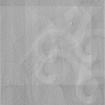
\includegraphics[width=\textwidth]{Chapters/flopt/Figs/PDF/results/helix/unfilttered_reconstruction_helix_iradon}
    \caption{Unfiltered reconstruction using a radon transform}
    \label{fig:unfilttered_reconstruction_helix_iradon}
  \end{subfigure}\hfill
  \begin{subfigure}[t]{0.3\textwidth}
    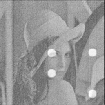
\includegraphics[width=\textwidth]{Chapters/flopt/Figs/PDF/results/helix/filtered_recon_helix}
    \caption{Filtered reconstruction using the new algorithm}
    \label{fig:filtered_recon_helix}
  \end{subfigure}
    \hfill
    \label{fig:flopts}
  \caption{Comparison of the two reconstructions under sample imaging with a systematic drift, in 3D though represented here in 2D.}
\end{figure}



%Textwidth is \the\textwidth


\todo{Flowchart of algorithm?}
\todo{Insert graph of reconstruction and line profiles for cases with rotation 2D + 3D + drift}
\todo{Insert graph of reconstruction using KNOWN R|T}


\section{Discussion}

Future work:
It is possible to use 3 separate views to reconstruct a scene, this involves quaternion tensors versus matrices.
The maths gets progressively harder but it is theoretically possible to input each view in directly into a special mathematical construct.
